\documentclass{article}

\usepackage{custom}

\usepackage[utf8]{inputenc} % allow utf-8 input
\usepackage[T1]{fontenc}    % use 8-bit T1 fonts
\usepackage{hyperref}       % hyperlinks
\usepackage{url}            % simple URL typesetting
\usepackage{booktabs}       % professional-quality tables
\usepackage{amsfonts}       % blackboard math symbols
\usepackage{nicefrac}       % compact symbols for 1/2, etc.
\usepackage{microtype}      % microtypography
\usepackage{lipsum}

\usepackage{graphicx}
\usepackage{listings}
\usepackage{color}

\definecolor{dkgreen}{rgb}{0,0.6,0}
\definecolor{gray}{rgb}{0.5,0.5,0.5}
\definecolor{mauve}{rgb}{0.58,0,0.82}

\lstset{frame=tb,
  aboveskip=3mm,
  belowskip=3mm,
  showstringspaces=false,
  columns=flexible,
  basicstyle={\small\ttfamily},
  numbers=none,
  numberstyle=\tiny\color{gray},
  keywordstyle=\color{blue},
  commentstyle=\color{dkgreen},
  stringstyle=\color{mauve},
  breaklines=true,
  breakatwhitespace=true,
  tabsize=4
}

\title{SST-SystemC Interoperability Toolkit}

\author{
  Sabbir Ahmed
}

\begin{document}
  \maketitle

  \begin{abstract}
    SST-SystemC Interoperability Toolkit (SSTSCIT) is a toolkit developed to provide interoperability between Structural Simulation Toolkit (SST) and SystemC. SST is a parallel event based simulation framework developed by Sandia National Laboratories that allows custom and vendor models to be interconnected to create a simulation environment. SystemC, by Accellera Systems Initiative, is a system-level modeling language composed of C++ classes and macros. SSTSCIT aims to provide the capability to interoperate the two systems without interfering with any of the kernels by concealing the communication protocols in black box interfaces.
  \end{abstract}

  \section{Introduction}
  % A toolkit to provide interoperability between Structural Simulation Toolkit (SST 8 with SST Elements 8) and SystemC 2.3 (with Transaction-Level Modeling Library (TLM 2)).

  This collection of header files provides methods to transmit and receive signals between SST components and SystemC modules. The toolkit provides a black box interface that can be interfaced with both SST and SystemC via their internal communication transports. 

  \begin{figure}[!h]
    \centering
    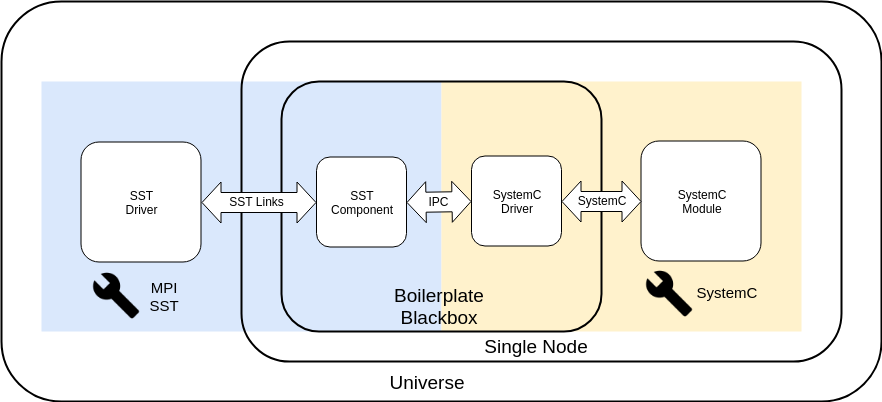
\includegraphics[width=6in]{comm.png}
    \caption{Components of SSTSCIT}
    \label{fig:fig1}
  \end{figure}

  \section{Components} \label{sec:comp}

    \subsection{Black Box Interface}
    The black box interface consists of:
    \begin{enumerate}
        \item A SystemC driver
        \item An SST component
    \end{enumerate}

    Each SystemC modules must have their corresponding driver file to interoperate within the black box interface. It is possible to interoperate multiple SystemC modules with a single driver file. However, the additional communication lines must be accounted for in the corresponding black box SST component.

    The toolkit includes a Python class that generates the boilerplate code required for the black box interface.

    \subsection{UML}

  \section{Communication} \label{sec:comm}

    \subsection{Inter-Black Box Communication}
    The two components inside the black box interface are spawned in the same node and therefore communicate via interprocess communication (IPC) transports. The following is a list of supported IPC transports:
    \begin{enumerate}
        \item Unix domain sockets
        \item ZeroMQ
    \end{enumerate}

    It is possible to add custom IPC protocols to the interface by implementing a derived class of \lstinline{sigutils::SignalIO} with customized sending and receiving methods.

    \subsection{SST-Black Box Communication}
    An SST model can interface the black box via standard SST links.

    The following snippets demonstrate an SST link transmitting a unidirectional signal from the SST environment to the black box interface.

\begin{lstlisting}[language=C++]
// parent_sst.cpp

// register a string event in the class declaration
SST_ELI_DOCUMENT_PORTS(
    { "demo_din", "Demo model data in", { "sst.Interfaces.StringEvent" }},
    ...
)

// initialize the link in the class declaration
SST::Link *demo_din;

// set up the SST link in the constructor
demo_din = configureLink("demo_din");

// trigger the event in the clocked function
demo_din->send(new SST::Interfaces::StringEvent(...));
\end{lstlisting}

\begin{lstlisting}[language=C++]
// blackboxes/demo.cpp

// register the same string event in the class declaration
SST_ELI_DOCUMENT_PORTS(
    { "demo_din", "Demo model data in", { "sst.Interfaces.StringEvent" }},
    ...
)

// initialize the same link in the class declaration
SST::Link *demo_din;

// set up the SST link in the constructor with an event handler
demo_din = configureLink(
    "demo_din",
    new SST::Event::Handler<demo>(this, &demo::handle_event)
);

// receive and parse the event in the event handler
void demo::handle_event(SST::Event *ev) {
    auto *se = dynamic_cast<SST::Interfaces::StringEvent *>(ev);
    if (se) {
        std::string _data_in = se->getString();
        ...
    }
    delete ev;
}
\end{lstlisting}

    \subsection{SystemC-Black Box Communication}
    A SystemC module can be interfaced by a standard source file inclusion.

  \section{Proof of Concept}

    \subsection{Car Wash}

    \subsection{Continuous Integration}

\end{document}
